\section{Sakupljač otpadaka}
\label{sec:djubretar}

Izvršavanje programa na računaru praćeno je stvaranjem brojnih struktura podataka (objekata).
Neke od njih generiše sam program, dok su druge vezane za njegovu implementaciju. Sve te strukture podataka se skladište u deo memorije koji se naziva heap.

\subsection{Sistem za upravljanje memorijom}
\label{subsec:sistem}

Osnovna gradivna jedinica heap-a je memorijska reč (\textit{memory word}). Jedna ili više reči  formiraju logičku celinu koja se naziva ćelija (\textit{cell}) (\ref{fig:slika 1}). Ona predstavlja osnovni element za skladištenje struktura podataka, što znači da se svaka struktura smešta u potreban broj ćelija.

\begin{figure}[h!]
\begin{center}
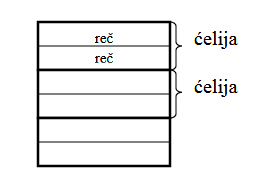
\includegraphics[scale=0.75]{celija.png}
\end{center}
\caption{Struktura heap-a}
\label{fig:slika 1}
\end{figure}

Deo operativnog sistema koji je zadužen za skladištenje struktura podataka u heap-u naziva se \textit{sistem za upravljanje memorijom} (\textit{memory manager}). Da bi neki objekat smestio u heap, on mora da:
\begin{itemize}
\item Odredi koliko je ćelija potrebno za skladištenje objekta
\item odredi konkretne ćelije koje će biti iskorišćene za to i
\item po završetku skladištenja, na neki način evidentira u kojim se ćelijama nalazi pomenuti objekat kako bi mu kasnije mogao pristupiti.
\end{itemize}
~
\\
\indent Ukoliko objekat više nije potreban programu, sistem za upravljanje memorijom
jednostavno uništi njegov koreni pokazivač i tako onemogući pristup ćelijama tog objekta. Ovakav način uništavanja nepotrebnih objekata je vrlo jednostavan za implementaciju, ali ima i jedan veliki nedostatak: ćelije koje su bile dodeljene objektu ne mogu se ponovo koristiti za smeštanje novih podataka, jer se ne nalaze u listi, odnosno steku slobodnih ćelija.
\\
Takve se ćelije nazivaju otpadak ili đubre (garbage) i moraju se reciklirati, tj. pretvoriti u slobodne.

\subsection{Sakupljač otpadaka sa brojanjem referenci}
\label{ref:reference counter}

Ideju za ovaj tip sakupljača otpadaka dao je Collins 1960.godine [Col60]. On se primenjuje u sistemima kod kojih je heap baziran na listi. Svaka ćelija u heap-u sadrži jednu reč koja se naziva brojač referenci. Vrednost te reči je broj referenci na ćeliju, tj. broj pokazivača koji na nju pokazuju. Kada se neki podatak smesti u ćeliju i ona postane aktivna, njen brojač referenci dobija vrednost 1. Ako u toku rada program kreira još neki pokazivač na tu ćeliju, njen brojač povećava vrednost za jedan. Ukoliko se uništi neki pokazivač na ćeliju, brojač smanjuje vrednost za jedan. Ako vrednost brojača postane nula, to znači da ne postoji nijedan pokazivač na tu ćeliju, tj. da joj se ne može pristupiti polazeći od nekog korenog pokazivača, pa ona više nije aktivna. Čim ćelija postane neaktivna, reciklira se i to tako što se povezuje u listu slobodnih ćelija. Ovim se izbegavaju dugotrajni procesi traženja aktivnih ćelija i recikliranja neaktivnih, koji su karakteristični za ostale tipove sakupljača otpadaka. Sve ovo omogućava da se recikliranje otpadaka obavlja paralelno sa izvršavanjem programa, pa je ovaj tip sakupljača pogodan za real-time sisteme.


%% George E. Collins. “A method for overlapping and erasure of lists”, Communications of the ACM,3(12):655-657, December 1960.
%% to je referenca za [Col60]
